\chapter{Optimización de Hiperparámetros}

\section{Planteo del Problema}

Sea $f: X \rightarrow \mathbb{R}$ una función que devuelve el máximo error de validación de un modelo entrenado a partir de una combinación de hiperparámetros $\textbf{x} \in X$, se desea encontrar $\hat{\textbf{x}}$:

\[
\textbf{x}^* = arg \min_{\textbf{x} \in X} f(\textbf{x})
\]

Es decir, se busca encontrar la combinación óptima de hiperparámetros dentro de un dominio $X$ para obtener el mínimo error de representación en un dado conjunto de validación. En el caso de la construcción de una base \textit{hp-greedy} óptima: 

\[
\textbf{x} = (n_{max}, l_{max}, \varepsilon, \hat{\Lambda}_0).
\]


%El hiperparámetro de mayor interés es sin duda la $semilla$, pues a primera vista no hay una forma obvia de elegir su valor óptimo. Además una semilla óptima para una combinación de $(n_{max_1}, l_{max_1})$ no lo será necesariamente para otra combinación $(n_{max_2}, l_{max_2})$.

%También se observó que en ciertas situaciones un valor muy elevado de $l_{max}$ o muy pequeño de la $tolerancia$ $greedy$ pueden conducir a un modelo \textit{sobreajustado}. Por esto es de interés realizar una optimización que involucre a la totalidad de los hiperparámetros dentro del dominio $X$. 


El problema al momento de realizar esta optimización es que la función $f$ no tiene una expresión analítica, sino es que es el resultado de entrenar el modelo y evaluar el error de representación con un conjunto de validación, lo que la hace costosa de evaluar (computacionalmente hablando). Este capítulo se centrará principalmente en la \textbf{optimización Bayesiana} \cite{7352306, https://doi.org/10.48550/arxiv.1012.2599}, un método que intenta reducir al mínimo el número de evaluaciones de $f$ para encontrar $\hat{\textbf{x}}$ y se puede colocar dentro de una categoría llamada optimización secuencial basada en modelos, o \textbf{SMBO}\cite{dewancker2015bayesian,NIPS2011_86e8f7ab} (\textit{Secuential Model-Based Optimization}).


Además existen dos métodos muy utilizados que no utilizan modelos, los cuales son la \textbf{busqueda exaustiva} (o \textit{grid search}) y la \textbf{búsqueda aleatoria}. Estos métodos se utilizaron en casos sencillos de optimización para realizar una comparación con la optimización bayesiana.


\subsubsection*{Comentario sobre el dominio $X$}


Si bien la tolerancia \textit{greedy} $\varepsilon$ puede tomar cualquier valor real no nulo (a diferencia de $n_{max}, l_{max}$ y $\hat{\Lambda}_0$ que toman valores discretos), para simplificar la búsqueda de $\hat{\textbf{x}}$ se utilizaron siempre distribuciones discretas en el espacio logarítmico. Más específicamente se utilizaron conjuntos de la forma $C = \{1\times 10^{t} \  | \ a \leq t \leq b,  t \in {\mathbb{Z}} \}$. De esta forma $X$ será un conjunto finito y estará definido por los valores extremos de cada hiperparámetro. 


\section{Optimización Bayesiana}

\begin{figure}[h!]
\centering
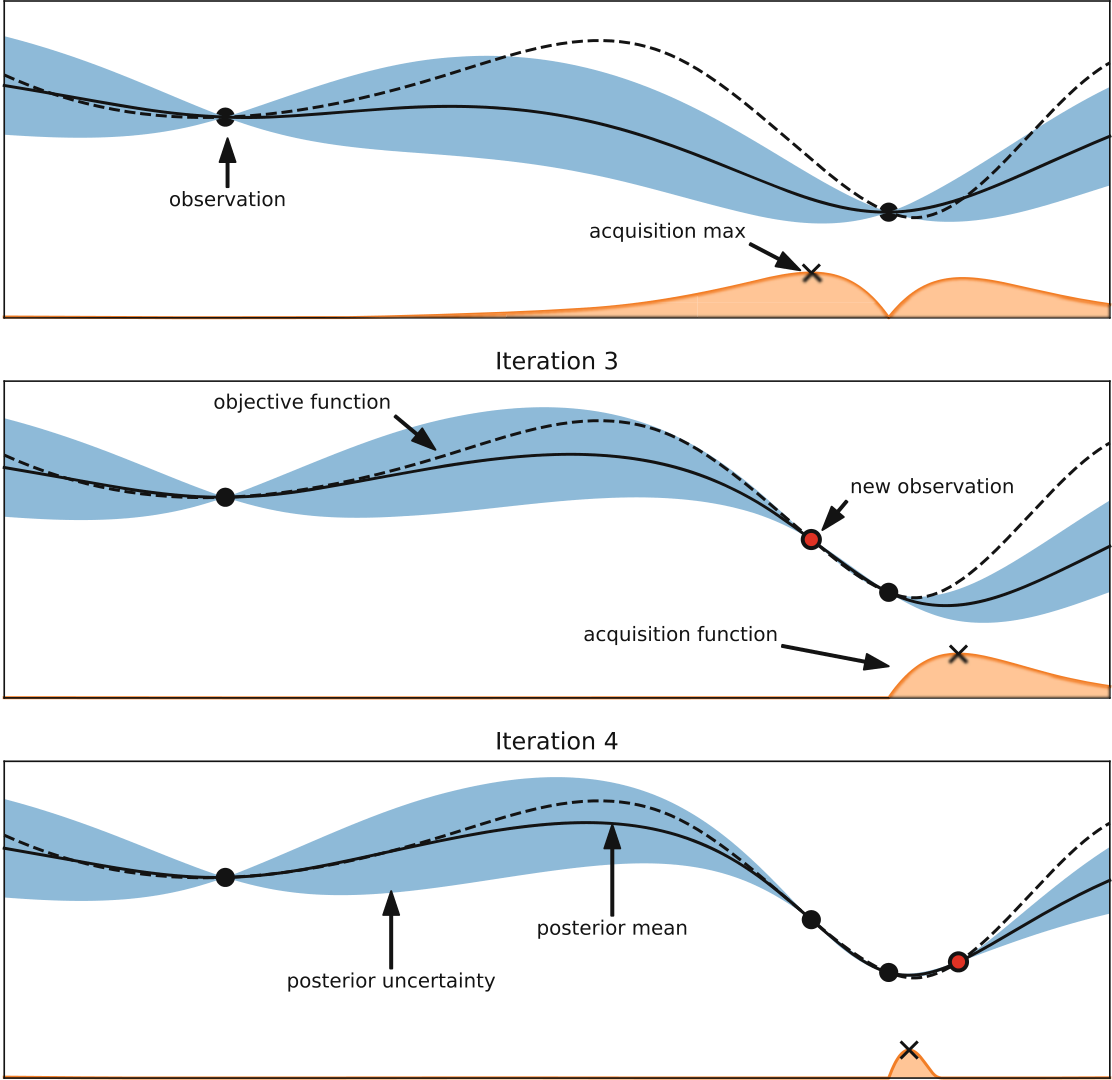
\includegraphics[width=.7\columnwidth]{bayesian.png}
\caption{En la figura se observan tres iteraciones de una optimización bayesiana para una función sencilla con parámetro unidimensional. En linea punteada está representada la función real, mientras que con linea gruesa se representa el valor medio del modelo estadístico (en este caso construido utilizando procesos gaussianos). El área pintada en azul representa la incertidumbre del modelo, que tiende a cero en los puntos que representan las observaciones realizadas. Debajo se puede ver una función de adquisición en color naranja, que indica el siguiente punto a evaluar \cite{Feurer2019}.}
\label{fig:bayesian}
\end{figure}

La optimización bayesiana es un método que utiliza la información de todas las evaluaciones realizadas de la función $f$ para decidir que valor de $\textbf{x}$ evaluar a continuación, reduciendo así el número necesario de evaluaciones de $f$ para encontrar el mínimo.

Para explicar como funciona este método se parte de un formalismo llamado optimización secuencial basada en modelos, que no es más que una generalización de la optimización bayesiana.

\subsection{Optimización Secuencial Basada en Modelos}

La idea es aproximar la función $f$ a partir de un modelo sustituto $\mathcal{M}$.

Se parte de un conjunto de observaciones $D = \{(\textbf{x}^{(1)},y^{(1)}), \cdots, (\textbf{x}^{(k)},y^{(k)}) \}$, donde $y^{(j)} = f(\textbf{x}^{(j)})$, a partir del cual se ajusta el modelo sustituto $\mathcal{M}$. Luego utilizando las predicciones del modelo se maximiza una función $S$ llamada función de adquisición que elije el siguiente conjunto de hiperparámetros $\textbf{x}_i \in X$ para evaluar la función $f$ y se agrega el par $(\textbf{x}_i, f(\textbf{x}_i))$ al conjunto de observaciones $D$. Una vez hecho esto se vuelve a ajustar el modelo $\mathcal{M}$ y se repite el proceso, que está explicado en forma de pseudocódigo en el algoritmo \ref{alg:SMBO}.

%En la optimización secuencial basada en modelos, cada evaluación de la función $f$ se decide en base a un conjunto $D$ de observaciones realizadas previamente. Esto se logra entrenando un modelo sustituto $\mathcal{M}$ en base al conjunto $D$, y luego utilizando una función $S$ llamada función de \textit{adquisición}, que decidirá el mejor punto a evaluar en la función real.

%Se parte de un conjunto $D = {(\textbf{x}}$ generado a partir de un muestreo de observaciones de la función $f$ de la forma $(\textbf{x}_j, f(\textbf{x}_j))$, a partir del cual se ajusta el modelo sustituto $\mathcal{M}$. Luego, maximizando la función de adquisición $S$ se elije el siguiente conjunto de hiperparámetros $\textbf{x}_i$ para evaluar la función $f$ y se agrega el par $(\textbf{x}_i, f(\textbf{x}_i))$ al conjunto de observaciones $D$. Una vez hecho esto se vuelve a ajustar el modelo $\mathcal{M}$ y se repite el proceso, que está explicado en forma de pseudocódigo en el algoritmo \ref{alg:SMBO}.


\begin{algorithm}
\caption{\texttt{SMBO}}
\label{alg:SMBO}
\begin{algorithmic}[1]
\Require $f, X, S,\mathcal{M}$
\State $D =$ InicializarMuestras$(f, X)$
\vspace{1mm}
\For{$i = 1, 2, ...$}
	\State $\mathcal{M} =$ AjustarModelo$(D)$
	\State $\textbf{x}_{i} = arg \max_{\textbf{x}\in X} \mathcal{S}(\textbf{x}, \mathcal{M})$ .
	\State $y_i = f(\textbf{x}_i)$	\Comment{Paso costoso}
	\State $D = D \cup \{(\textbf{x}_i, y_i)\}$
\EndFor
\vspace{3mm}

\end{algorithmic}
\end{algorithm}

\subsection*{Optimización Bayesiana}

Lo que caracteriza a la optimización bayesiana dentro del formalismo de la optimización secuencial basada en modelos, es justamente la creación del modelo.
En la optimización bayesiana se construye un modelo estadístico, donde se representa con  $P(y|\textbf{x})$ la predicción del modelo, siendo $y$ el resultado de una evaluación $f(\textbf{x})$. El nombre del método se debe a que para la construcción del modelo se utiliza el teorema de Bayes:
  
 \[
 P(y|\textbf{x}) = \frac{P(\textbf{x}|y) \ P(y)}{P(\textbf{x})}
 \]
 
 En la terminología bayesiana, se conoce a $P(y|\textbf{x})$ como probabilidad a posteriorí o \textit{posterior}, que es proporcional a la probabilidad a priori o \textit{prior} $P(y)$ por la función de verosimilitud o \textit{likelihood} $P(\textbf{x}|y)$. La probabilidad $P(\textbf{x})$ es una probabilidad marginal que sirve como factor de normalización, por lo que no es de tanto interés.


\subsubsection*{Procesos Gaussianos}

\begin{figure}[h!]
\centering
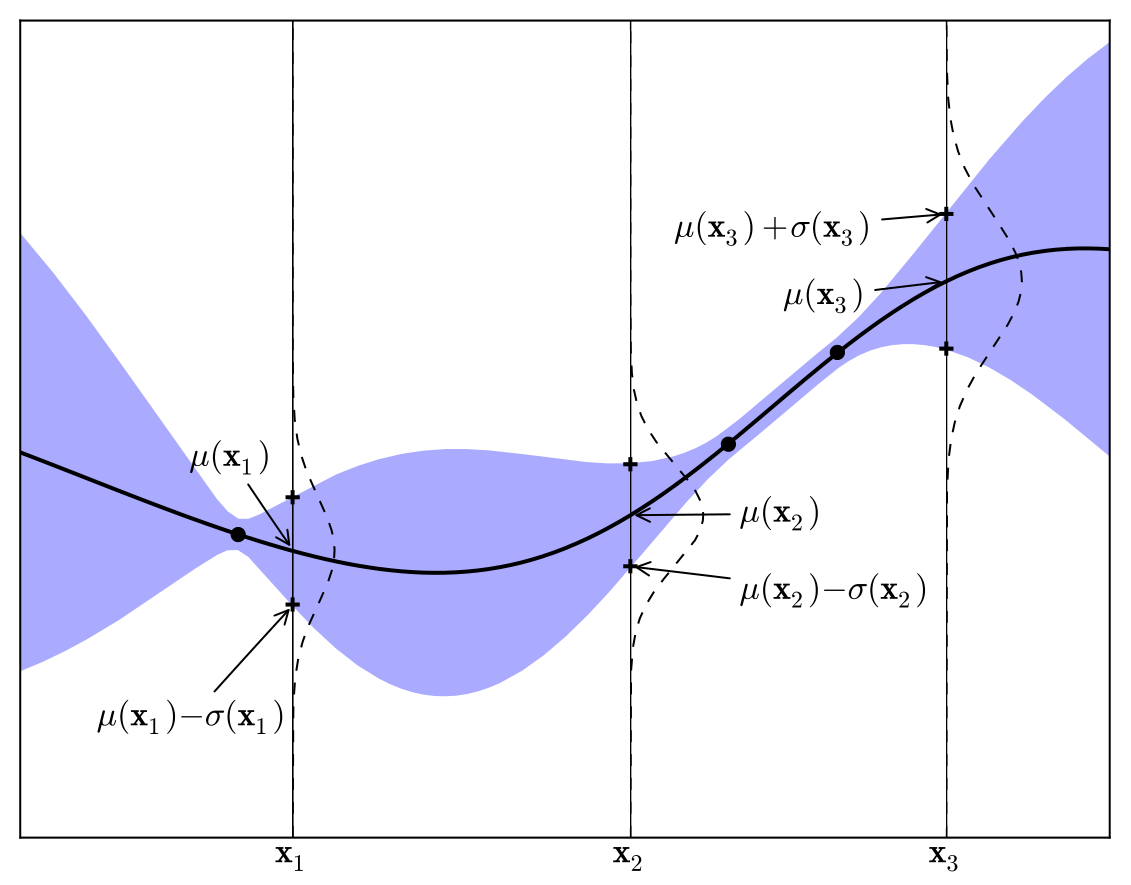
\includegraphics[width=.8\columnwidth]{gaussian.png}
\caption{Proceso Gaussiano unidimensional con tres observaciones representadas por los puntos negros. La linea gruesa representa la media del modelo predictivo y la zona azul la varianza en cada caso. Se representa con linea de trazo las distribuciones normales para los valores $x_1, x_2,$ y $x_3$\cite{https://doi.org/10.48550/arxiv.1012.2599}.}
\label{fig:gaussian}
\end{figure}

Una opción muy utilizada para la construcción del \textit{prior} y actualización del \textit{posterior} son los procesos gaussianos. Una forma sencilla de entender un proceso gaussiano es pensarlo como una función que para cada valor de $x$ devuelve la media $\mu(x)$ y la varianza $\sigma(x)$ de una distribución normal, en el caso particular de que $x$ sea unidimensional (ver figura \ref{fig:gaussian}). Con $\textbf{x}$ multidimensional, se obtiene una distribución normal multivariante, caracterizada por el vector $\bm{\mu}(\textbf{x})$ y la matriz de covarianza $\Sigma(\textbf{x}, \textbf{x}')$.

Sin embargo en este trabajo no se utilizan procesos gaussianos, principalmente porque parten del supuesto de que $f$ es continua. Para una introducción a la optimización bayesiana con procesos gaussianos ver \cite{https://doi.org/10.48550/arxiv.1012.2599}.

\subsection{Mejora Esperada: Función De Adquisición} 
 
%Debido a que la función $f$ no será necesariamente convexa, y seguramente tendrá varios mínimos locales, es necesario mantener un equilibrio entre la explotación y la exploración, es decir, explorar los mínimos tentativos sin dejar de lado las zonas inexploradas, en donde podría haber algún mínimo por descubrir. De esto se encarga la función de adquisición.
Para la elección de los puntos a evaluar en la función real se maximiza la función de adquisición $S$. Existen varias propuestas de funciones de adquisición, pero en este caso se utiliza la \textbf{mejora esperada} o EI(\textit{Expected Improvement}) \cite{EI1}. Sea $y^*$ un valor de referencia, se define a la mejora esperada  con respecto a $y^*$ como:


\begin{equation}
\label{eq:ei_def}
EI_{y^*}(\textbf{x}) := \int_{-\infty}^{\infty} \max(y^*-y,0) p(y|\textbf{x}) \ dy
\end{equation}
 

\subsection{Estimador de Parzen con Estructura Arbórea} 

 El estimador de Parzen con estructura arbórea o \textbf{TPE} (\textit{Tree-Structured Parzen Estimator}) \cite{NIPS2011_86e8f7ab} es una estrategia que modela $P(x_i|y)$ para cada $x_i \in X_i$ (es decir, que $x_i$ representa a cada hiperparámetro por separado) a partir de dos distribuciones creadas a utilizando las observaciones $D$:

\begin{equation}
\label{eq:tpe}
P(x_i|y) =
	\begin{cases}
		\ell (x_i) & \text{si } y <y^{*} \\
		g(x_i) & \text{si } y \geq y^{*},
	\end{cases}
\end{equation}


Donde las densidades $\ell(x_i)$ y $g(x_i)$ se construyen a partir de dos conjuntos $D_{\ell}$ y $D_g$, ambos subconjuntos de $D$, tal que $D_{\ell}$ contiene todas las observaciones con $y < y^*$, y $D_g$ contiene a todo el resto de forma que $D = D_{\ell} + D_g$. El valor de referencia $y^{*}$ será un valor por encima del mejor valor observado de $f(\textbf{x})$, que se selecciona para ser un cuantil $\gamma \in (0,1)$ de los valores observados $y$ tal que $P(y<y^{*}) = \gamma$.


\subsubsection*{Mejora Esperada con TPE}
Aplicando la ecuación \eqref{eq:tpe} a la definición de mejora esperada \eqref{eq:ei_def} se obtiene la siguiente relación \cite{NIPS2011_86e8f7ab}:

\begin{equation}
EI_{y^*}(x_i) \propto \left( \gamma + (1-\gamma) \frac{g(x_i)}{\ell (x_i)} \right)^{-1}
\end{equation}

Es decir que para maximizar la mejora esperada se debe escoger un valor $x_i$ que maximice el cociente $\ell(x_i)/g(x_i)$ (o minimice $g(x_i)/\ell(x_i)$).

\subsubsection*{Estimación de las Densidades}

Las densidades de probabilidad se estiman utilizando ventanas de Parzen. Sea $D_x = \{x_i \ | \ (\textbf{x}, y) \in D_{\ell} \ (o\ D_g) \}$:

\begin{equation}
P(x_i) = \frac{\sum_{x_i'\in D_x}w_{x_i'}k(x_i, x_i') + w_p k(x_i, x_p) }{\sum_{x_i'\in D_x}w_{x_i'}+w_p},
\end{equation}
 

donde $w_{x_i'}$ es el peso de la observación $x_i'$(ver \cite{https://doi.org/10.48550/arxiv.1209.5111}), $x_p$ es un valor fijo \textit{prior}, $w_p$ es un peso \textit{prior} (por defecto igual a $1$) y $k$ es la función \textit{kernel}, que en este caso son distribuciones gaussianas truncadas centradas en los puntos $x_i'$ (ver \cite{10.1145/3377930.3389817} para más detalle).

%LEER https://tech.preferred.jp/en/blog/multivariate-tpe-makes-optuna-even-more-powerful/ !!!

\subsection*{Algoritmo}

Finalmente se puede ver el procedimiento completo del estimador de Parzen con estructura arbórea en el algoritmo \ref{alg:TPE}. Un detalle importante es que el algoritmo requiere un valor $n_c$, que es el número de candidatos que se utilizarán para maximizar el cociente $\ell(x_i)/g(x_i)$ (es decir, para maximizar la función de adquisición). En la linea 6 del algoritmo se realiza el muestro de los $n_c$ candidatos, utilizando la distribución $\ell(x_i)$, para luego seleccionar $x_i^*$ a partir del conjunto $C_i$.
Para este trabajo se utilizó la implementación de este algoritmo realizada en el paquete \textbf{\textit{Optuna}} \cite{optuna_2019} escrito en el lenguaje de programación Python.

\begin{algorithm}
\caption{\texttt{TPE}}
\label{alg:TPE}
\begin{algorithmic}[1]
\Require
\begin{tabular}{c}
$D = \{(\textbf{x}^{(1)},y^{(1)}), \cdots, (\textbf{x}^{(k)},y^{(k)}) \}$ \Comment{Observaciones}  \\ 
$n_t \in \mathbb{N}$ \Comment{número de iteraciones} \\ 
$n_c \in \mathbb{N}$ \Comment{número de candidatos} \\
$\gamma \in (0,1) $ \Comment{cuantil para obtener $y^*$}
\end{tabular} 

\vspace{1mm}
\For{$t = 1, 2, ..., n_t$}
	\State $D_{\ell} = \{ (\textbf{x}, y) \in D | y < y^*, \ \text{con } P(y<y^*) = \gamma  \}$
	\State $D_g = D - D_{\ell}$
	\For{$x_i = n_{max}, l_{max}, \varepsilon ,...$} \Comment{Para cada hiperparámetro}
		\State Construir $\ell(x_i)$ con $\{x_i \ | \ (\textbf{x}, y) \in D_{\ell}\}$ y $g(x_i)$ con $\{x_i \ | \ (\textbf{x}, y) \in D_g \}$.
		\State $C_i = \{ x_i^{(j)} \sim \ell(x_i)| j=1, ..., n_c \}$ \Comment{muestreo de $n_c$ candidatos para $x_i^*$}
		\State $x_{i}^* = arg \max_{x_i\in C_i} \ell(x_i)/g(x_i)$
	\EndFor
	\State $D = D \cup \{(\textbf{x}^*, f(\textbf{x}^*)\}$ \Comment{$\textbf{x}^*$ es el vector construido a partir de cada $x_i$.}
\EndFor
\Ensure $\textbf{x}$ con el mínimo valor $y$ en $D$.
\vspace{3mm}

\end{algorithmic}
\end{algorithm}
 
 
 
 
\subsubsection*{TPE Multivariante} 

Una alternativa al algoritmo \ref{alg:TPE} es el algoritmo \textbf{TPE Multivariante}, implementado en Optuna \footnote{El algoritmo TPE Multivariante fue introducido en la siguiente actualización de Optuna: \url{https://github.com/optuna/optuna/pull/1767}}. La única diferencia es que en este caso las densidades no se construyen para cada hiperparámetro por separado, sino que se utilizan ventanas de Parzen multivariadas, dónde las funciones \textit{kernel} ahora son distribuciones gaussianas multivariadas. Es decir que en lugar de construir $\ell(x_i)$ y $g(x_i)$ para cada hiperparámetro, ahora se construye directamente $\ell(\textbf{x})$ y $g(\textbf{x})$.


\section{Resultados}


\subsection{Conjunto pequeño: Comparación de métodos}


\begin{figure}[h!]
\centering
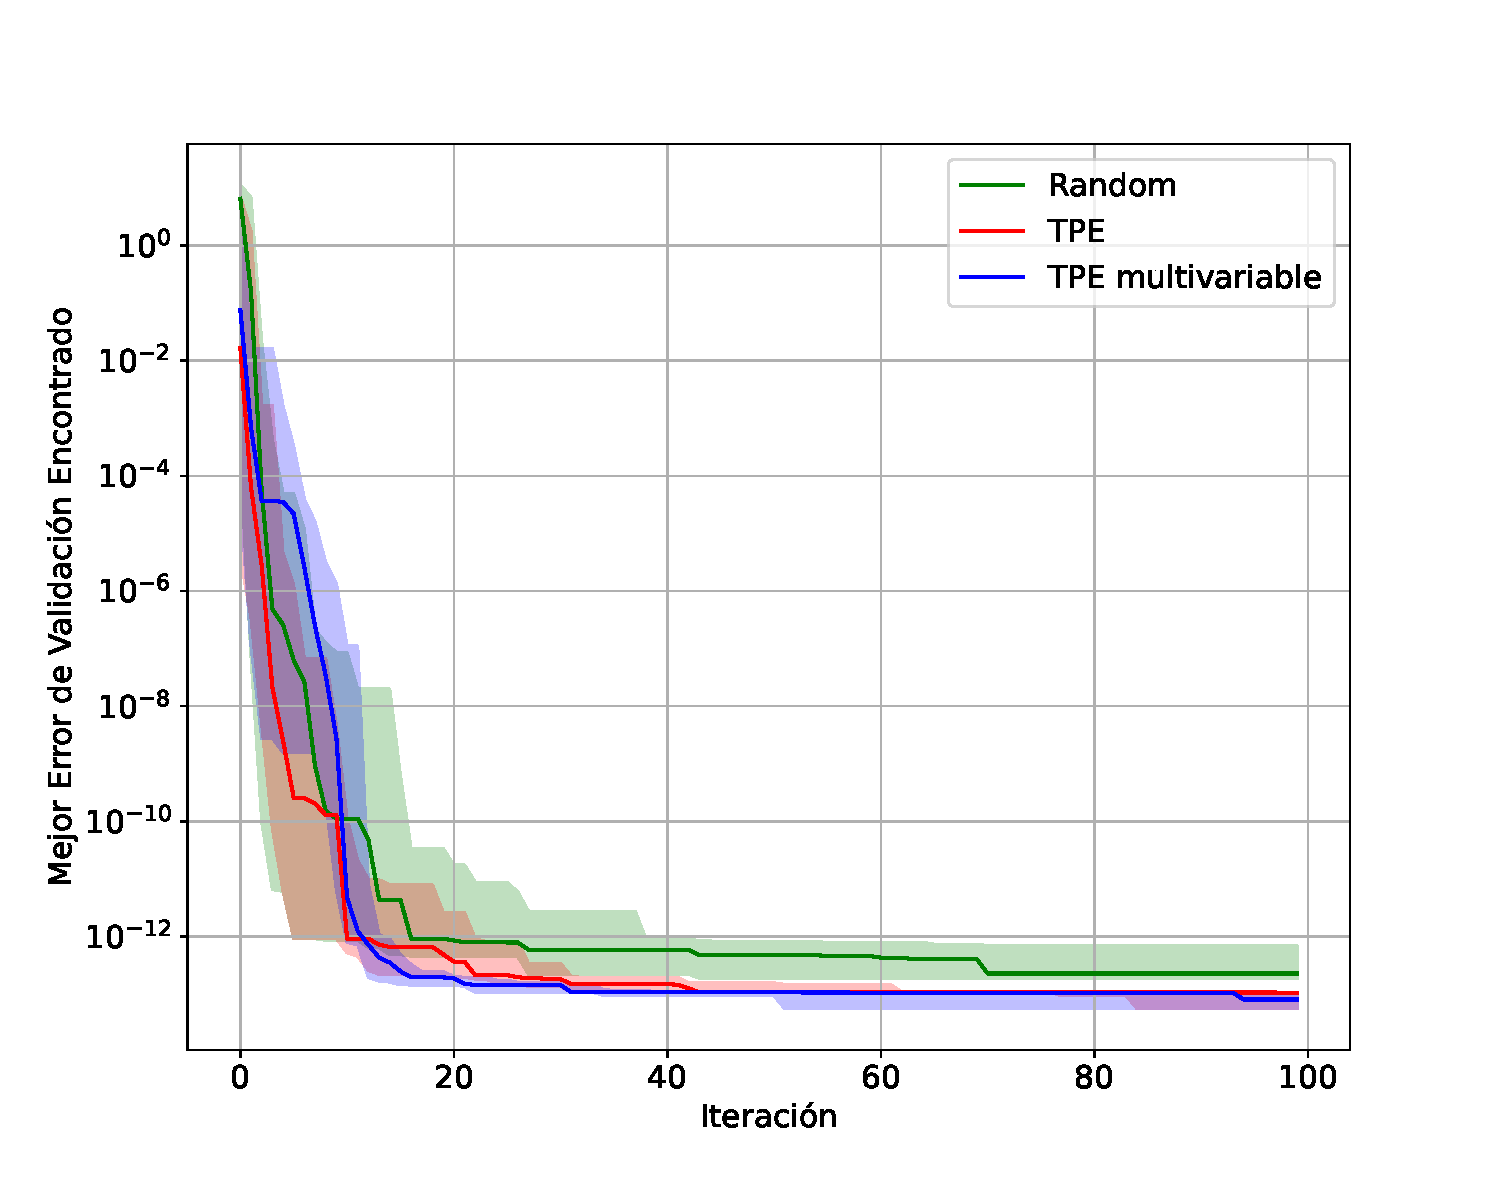
\includegraphics[width=.9\columnwidth, trim={1cm, 1cm, 1cm, 1.1cm}]{benchmark_0.pdf}
\caption{Comparación de convergencia. Se muestran los cuartiles para 20 optimizaciones realizadas, en cada caso.}
\label{fig:bench0}
\end{figure}

Utilizando un conjunto de entrenamiento con cien ondas equidistantes en el espacio del parámetro unidimensional $q: 1 < q < 8$, se quiere optimizar el error de representación para un conjunto de validación con quinientas ondas (cinco veces más denso). Los hiperparámetros a optimizar son $\textbf{x} = (n_{max}, l_{max}, \hat{\Lambda}_0)$, dejando $\varepsilon$ fijo en $1\times 10^{-12}$ para simplificar la búsqueda, que se realiza en los siguientes intervalos:

\begin{align*}
n_{max} &\in \{5, 6, 7, ..., 20\},\\
l_{max} &\in \{1, 2, 3, ..., 10 \},\\
\hat{\Lambda}_0 &\in \{q_0 \ | \ q_0 = 1 + i \Delta q, \ i\in \mathbb{N} : 0 \le i \le 99, \ \Delta q = 7/99 \}.
\end{align*}

Son 16 valores de $n_{max}$, 10 valores de $l_{max}$ y 100 para $q_0$ ($\hat{\Lambda}_0 = q_0$). Lo que hace un total de 16000 combinaciones posibles.

En la figura \ref{fig:bench0} se puede ver el resultado de realizar 20 optimizaciones de 100 iteraciones con tres diferentes métodos; búsqueda aleatoria (\textit{random}), TPE y TPE multivariante (los tres métodos están implementados en Optuna \cite{optuna_2019}). En linea oscura se representa la media del mejor error a cada iteración, y la zona sombreada representa los cuartiles. Aparte, en linea de trazo se marca el mejor error obtenido realizando una búsqueda exhaustiva (\textit{grid search}).


En las primeras 10 repeticiones los tres métodos son equivalentes, pues para el algoritmo TPE (tanto el normal como el multivariable) se parte de un muestreo aleatorio de 10 observaciones. En la figura \ref{fig:bench0} se ve claramente que luego de las décima iteración se produce el cambio más notorio entre los tres métodos. Gráficamente se puede ver que ambas versiones del algoritmo TPE dan un mejor resultado que la búsqueda aleatoria, pero aparte de esto se pueden utilizar métricas como el \textbf{mejor valor encontrado} para la mediana de $y$ o el \textbf{área bajo la curva} o \textbf{AUC} (\textit{Area Under the Curve})\cite{Dewancker2016ASF}. En la tabla \ref{tab:comp1} están los resultados de estas métricas, considerando solo las últimas 90 iteraciones.


\begin{table}
\centering
\begin{tabular}{@{}lccc@{}}
\toprule
\textbf{Algoritmo} & AUC (Mediana) & Mejor $Mediana(y)$ encontrada \\ 
\midrule
Búsqueda Aleatoria & $2.59\times 10^{-10}$ & $2.26\times 10^{-13}$ \\ 
TPE & $1.20\times 10^{-11}$ & $1.04\times 10^{-13}$ \\ 
TPE Multivariante & $5.20\times 10^{-12}$ & $5.48\times 10^{-14}$ \\ 
\bottomrule
\end{tabular} 
\caption{Comparación entre algoritmos de optimización.}
\label{tab:comp1}
\end{table}

\subsubsection*{Búsqueda Exhaustiva}
La búsqueda exhaustiva o \textit{grid search} consiste en probar todas las combinaciones posibles dentro de un espacio de hiperparámetros para seleccionar la solución óptima. Es decir que si se quiere buscar la combinación óptima de $(n_{max}, l_{max})$ para un rango de valores $n_{max} \in N,$ $l_{max} \in L$ se deberán probar todas las combinaciones posibles del producto cartesiano $N \times L = \{(n_{max}, l_{max}) | n_{max} \in N, l_{max} \in L\}$. 

\begin{figure}[h!]
\centering
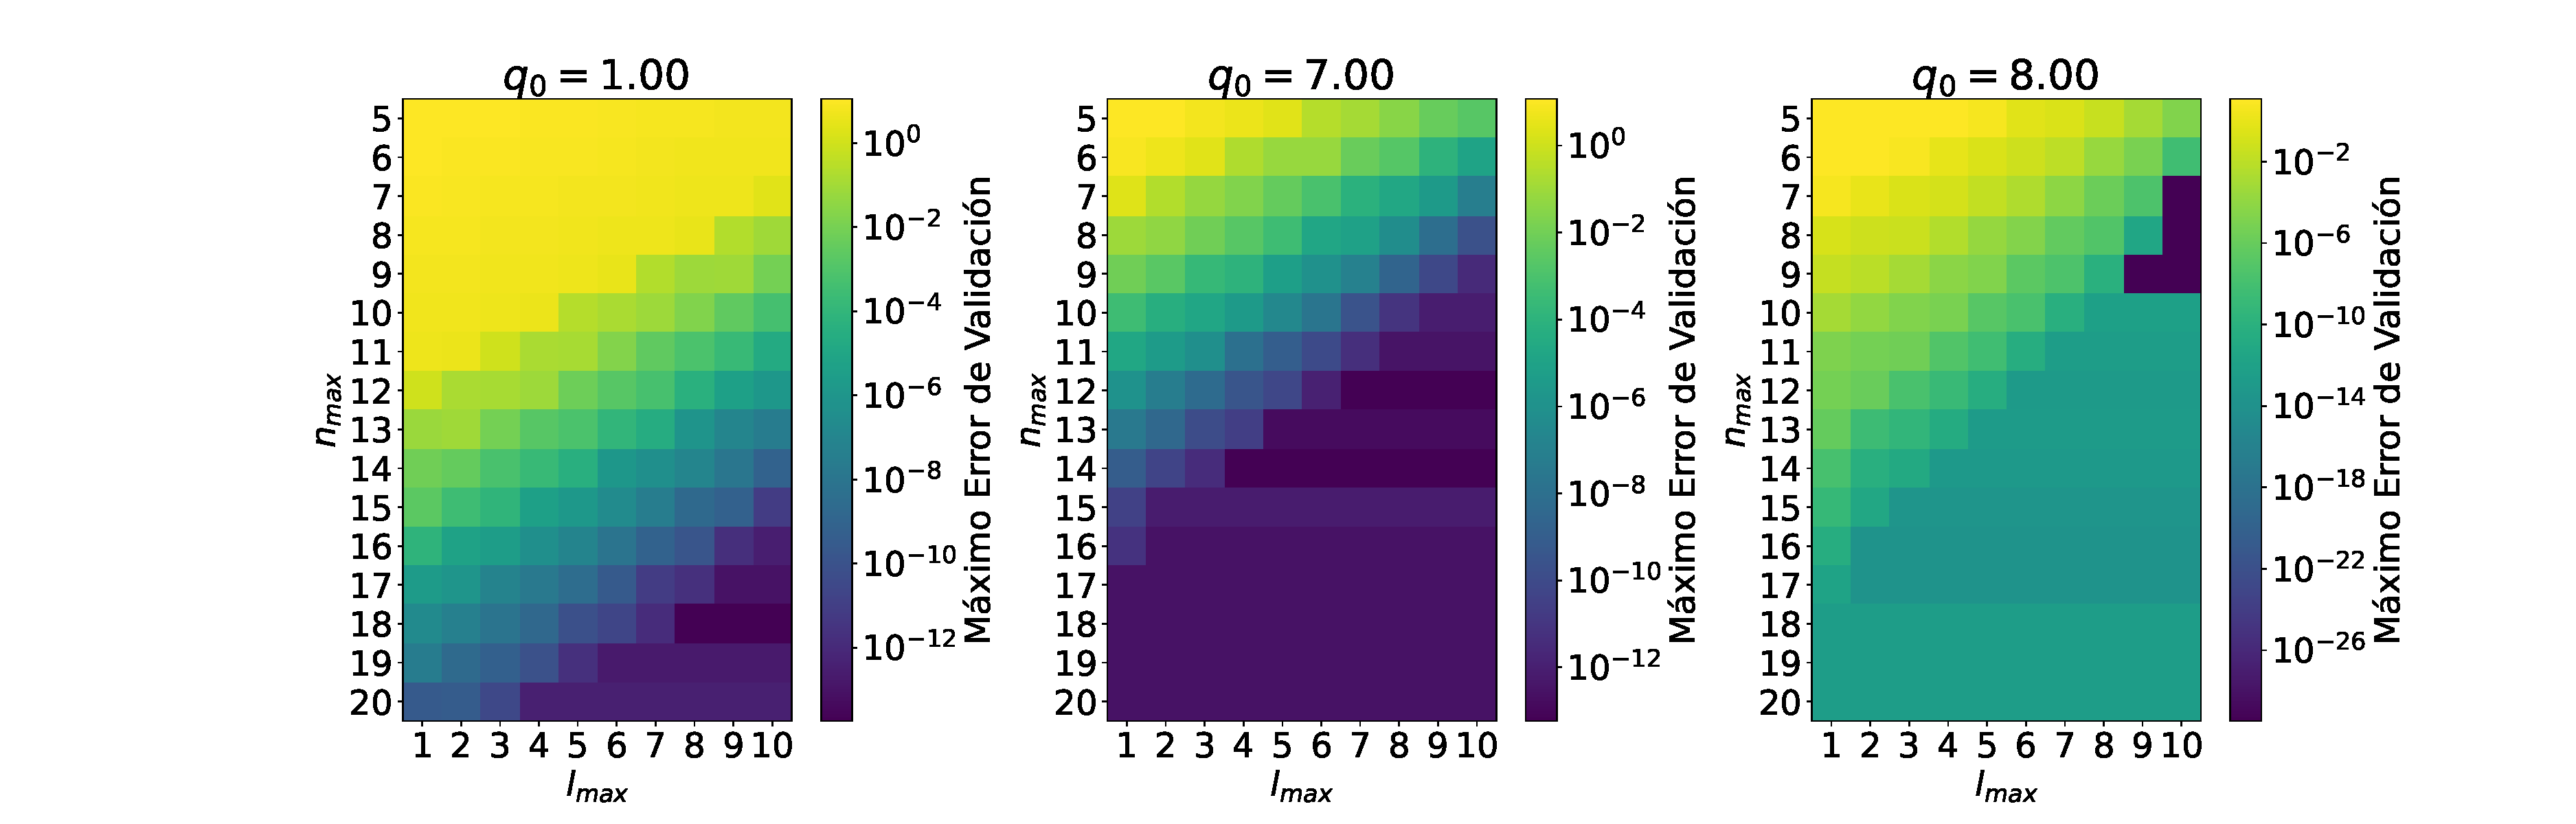
\includegraphics[width=1.05\columnwidth, trim={8cm, 1cm, 5cm, 1.1cm}]{grid_3_seeds.pdf}
\caption{Máximo error de validación en función de $n_{max}$ y $l_{max}$ para tres diferentes semillas $q_0$. }
\label{fig:grid_3_seeds}
\end{figure}

\begin{figure}[h!]
\centering
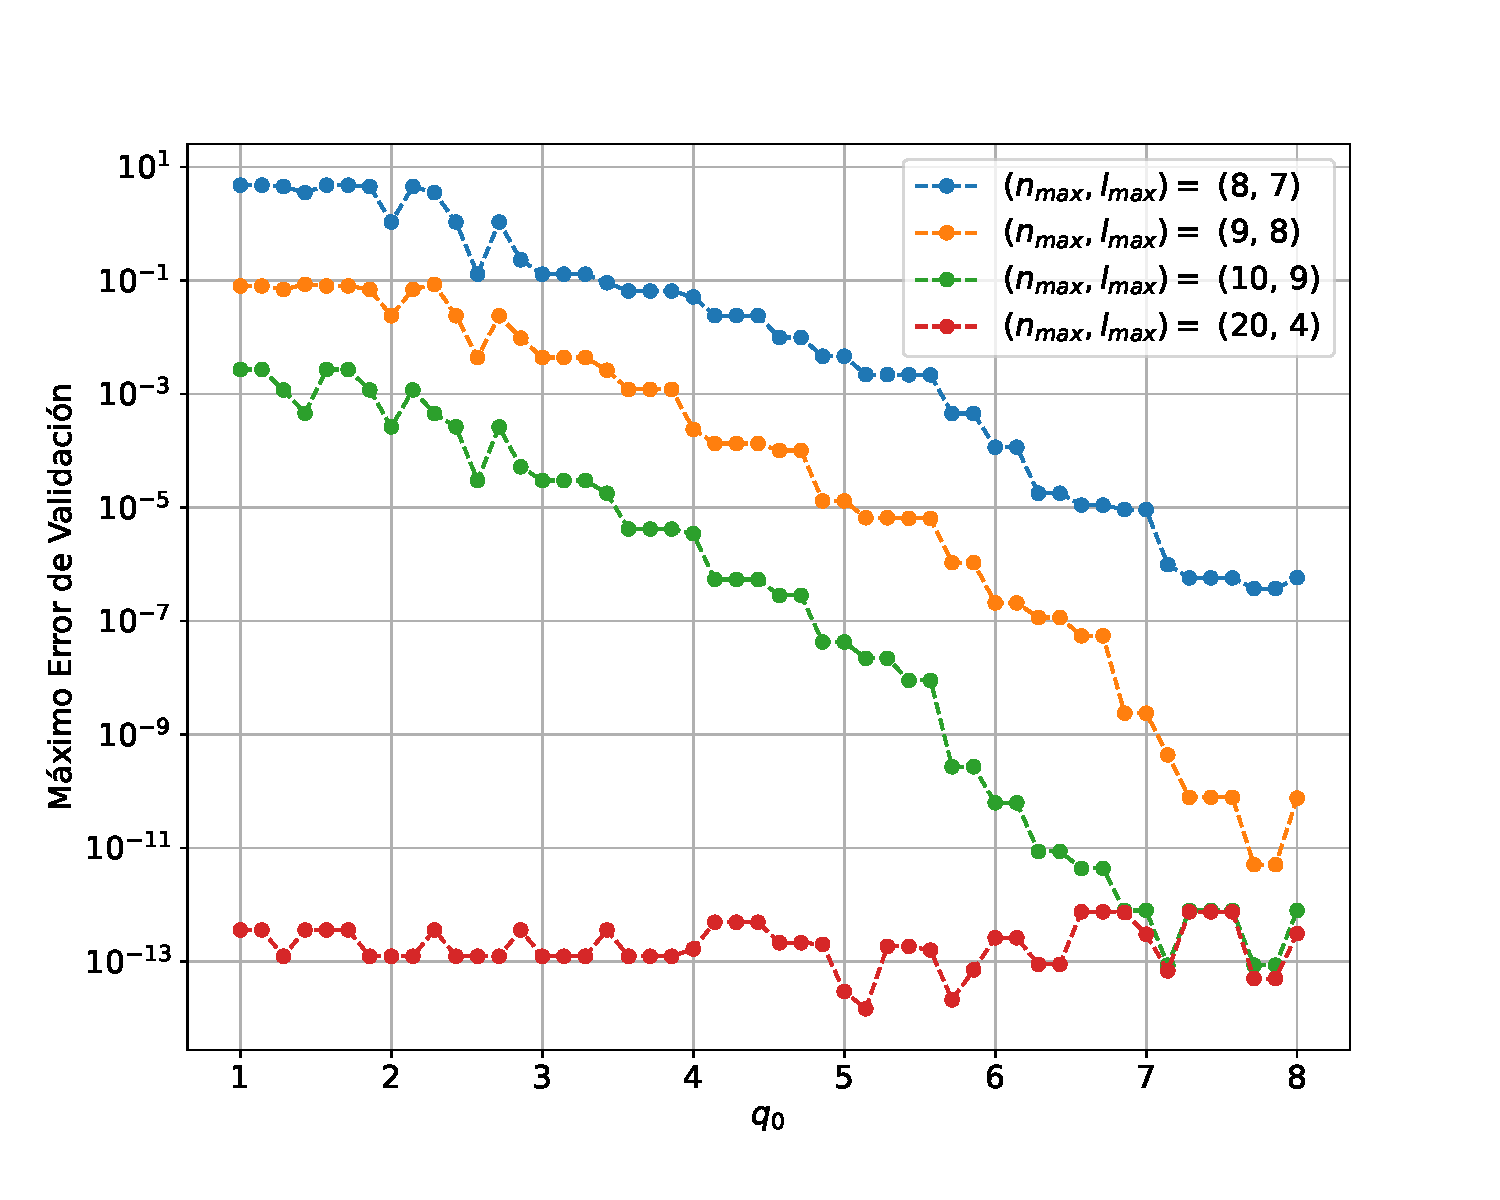
\includegraphics[width=.8\columnwidth, trim={1.1cm, 1cm, 1cm, 1.2cm}]{grid_seeds_0.pdf}
\caption{Máximo error de validación en función de la semilla $q_0$ para distintas combinaciones de $(n_{max}, l_{max})$}
\label{fig:grid_seed_0}
\end{figure}


 
%La ventaja de este método está en que el resultado óptimo está garantizado, pues se pueden comparar todos los resultados entre sí y elegir el mejor. El problema es que, como se mencionó, la función $f$ es costosa de evaluar, y por otro lado el número de combinaciones posibles escala exponencialmente con cada hiperparámetro extra a optimizar (además se debe tener en cuenta que la semilla $\hat{\Lambda}_0$ tendrá generalmente más de una dimension).

%Por estas razones la búsqueda exhaustiva no será un método viable en la mayoría de los casos que son de interés para este trabajo. Sin embargo se puede poner a prueba con casos simplificados para luego comparar los resultados con otros métodos más eficaces.

Si bien no se puede graficar el error en función de los tres hiperparámetros a la vez, se puede obtener bastante información al dejar fijo uno o dos hiperparámetros. Por ejemplo en la figura \ref{fig:grid_3_seeds} se observa el error de validación en función de las combinaciones posibles de  $n_{max}$ y $l_{max}$ para tres diferentes semillas. 

Luego en la figura \ref{fig:grid_seed_0} se ven los resultados de variar únicamente la semilla para diferentes combinaciones de $n_{max}$ y $l_{max}$. 
En este conjunto de datos se observa que para $(n_{max}, l_{max})=(20, 10)$ hay una diferencia de 9 ordenes de magnitud entre la peor y la mejor semilla (datos en color verde). Sin embargo para $(n_{max}, l_{max})=(15, 10)$ la diferencia es de 13 ordenes de magnitud (datos de color azul). Además el valor óptimo de la semilla no coincide exactamente en estos dos ejemplos, aunque tengan un comportamiento similar. Es decir que la influencia de la semilla depende del resto de hiperparámetros, sobre todo se tiene que tener en cuenta que en este caso la tolerancia \textit{greedy} tenía un valor $\varepsilon = 1\cdot 10^{-12}$, por lo que no se va a obtener un resultado mucho mejor que este.

\begin{figure}[h!]
\centering
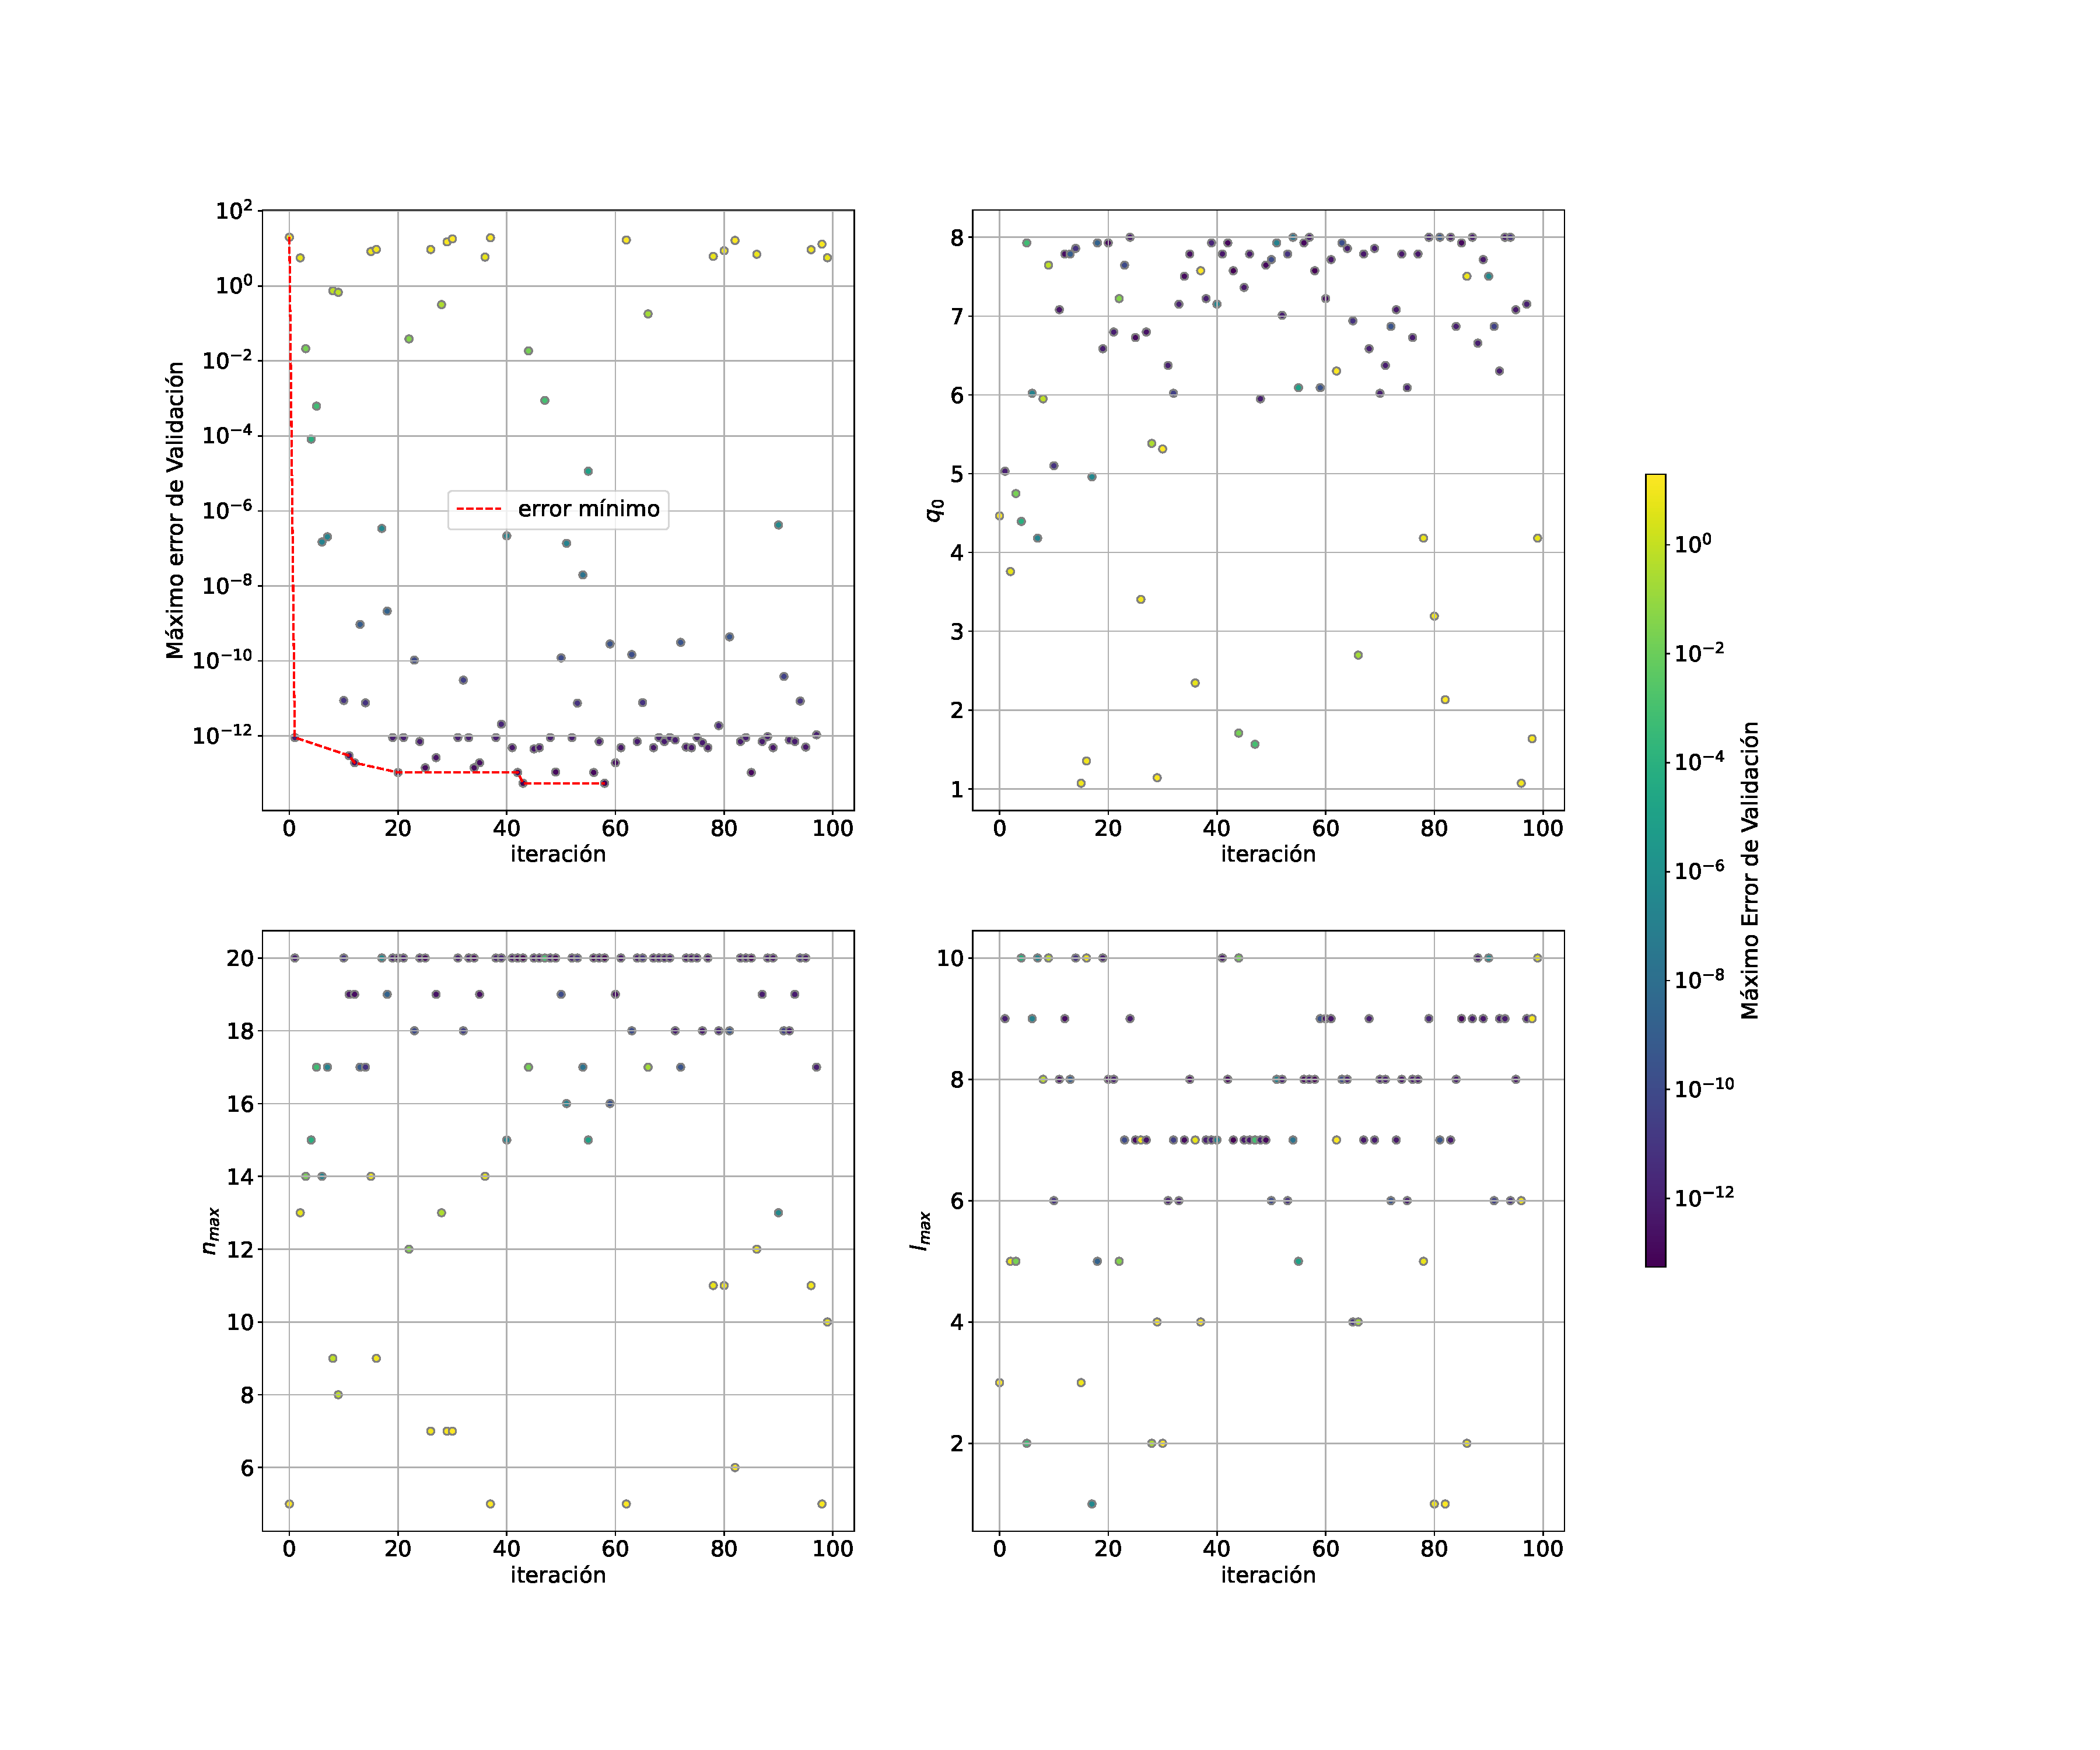
\includegraphics[width=1\columnwidth, trim={5cm, 5cm, 11cm, 5cm}]{Optuna_1d_simple.pdf}
\caption{Optimización con 100 iteraciones utilizando el algoritmo TPE multivariante para el conjunto de entrenamiento con semilla unidimensional.}
\label{fig:optuna_1d}
\end{figure}

\subsubsection*{Tiempo de Optimización}

Si bien la búsqueda exhaustiva garantiza encontrar el mejor resultado posible dentro del espacio de búsqueda, el tiempo necesario para realizar la búsqueda hace que el método no sea aplicable a casos relativamente complejos. En este caso sencillo, con 16000 combinaciones, la búsqueda requirió \textbf{25 horas} para completarse. En cambio las optimizaciones realizadas utilizando los algoritmos TPE tardaron una media de \textbf{8 minutos}.

Por último en la figura \ref{fig:optuna_1d} se puede ver gráficamente el proceso de optimización utilizando el algoritmo TPE multivariable.

\subsection{Optimización Completa}

\begin{figure}[p!]
\centering
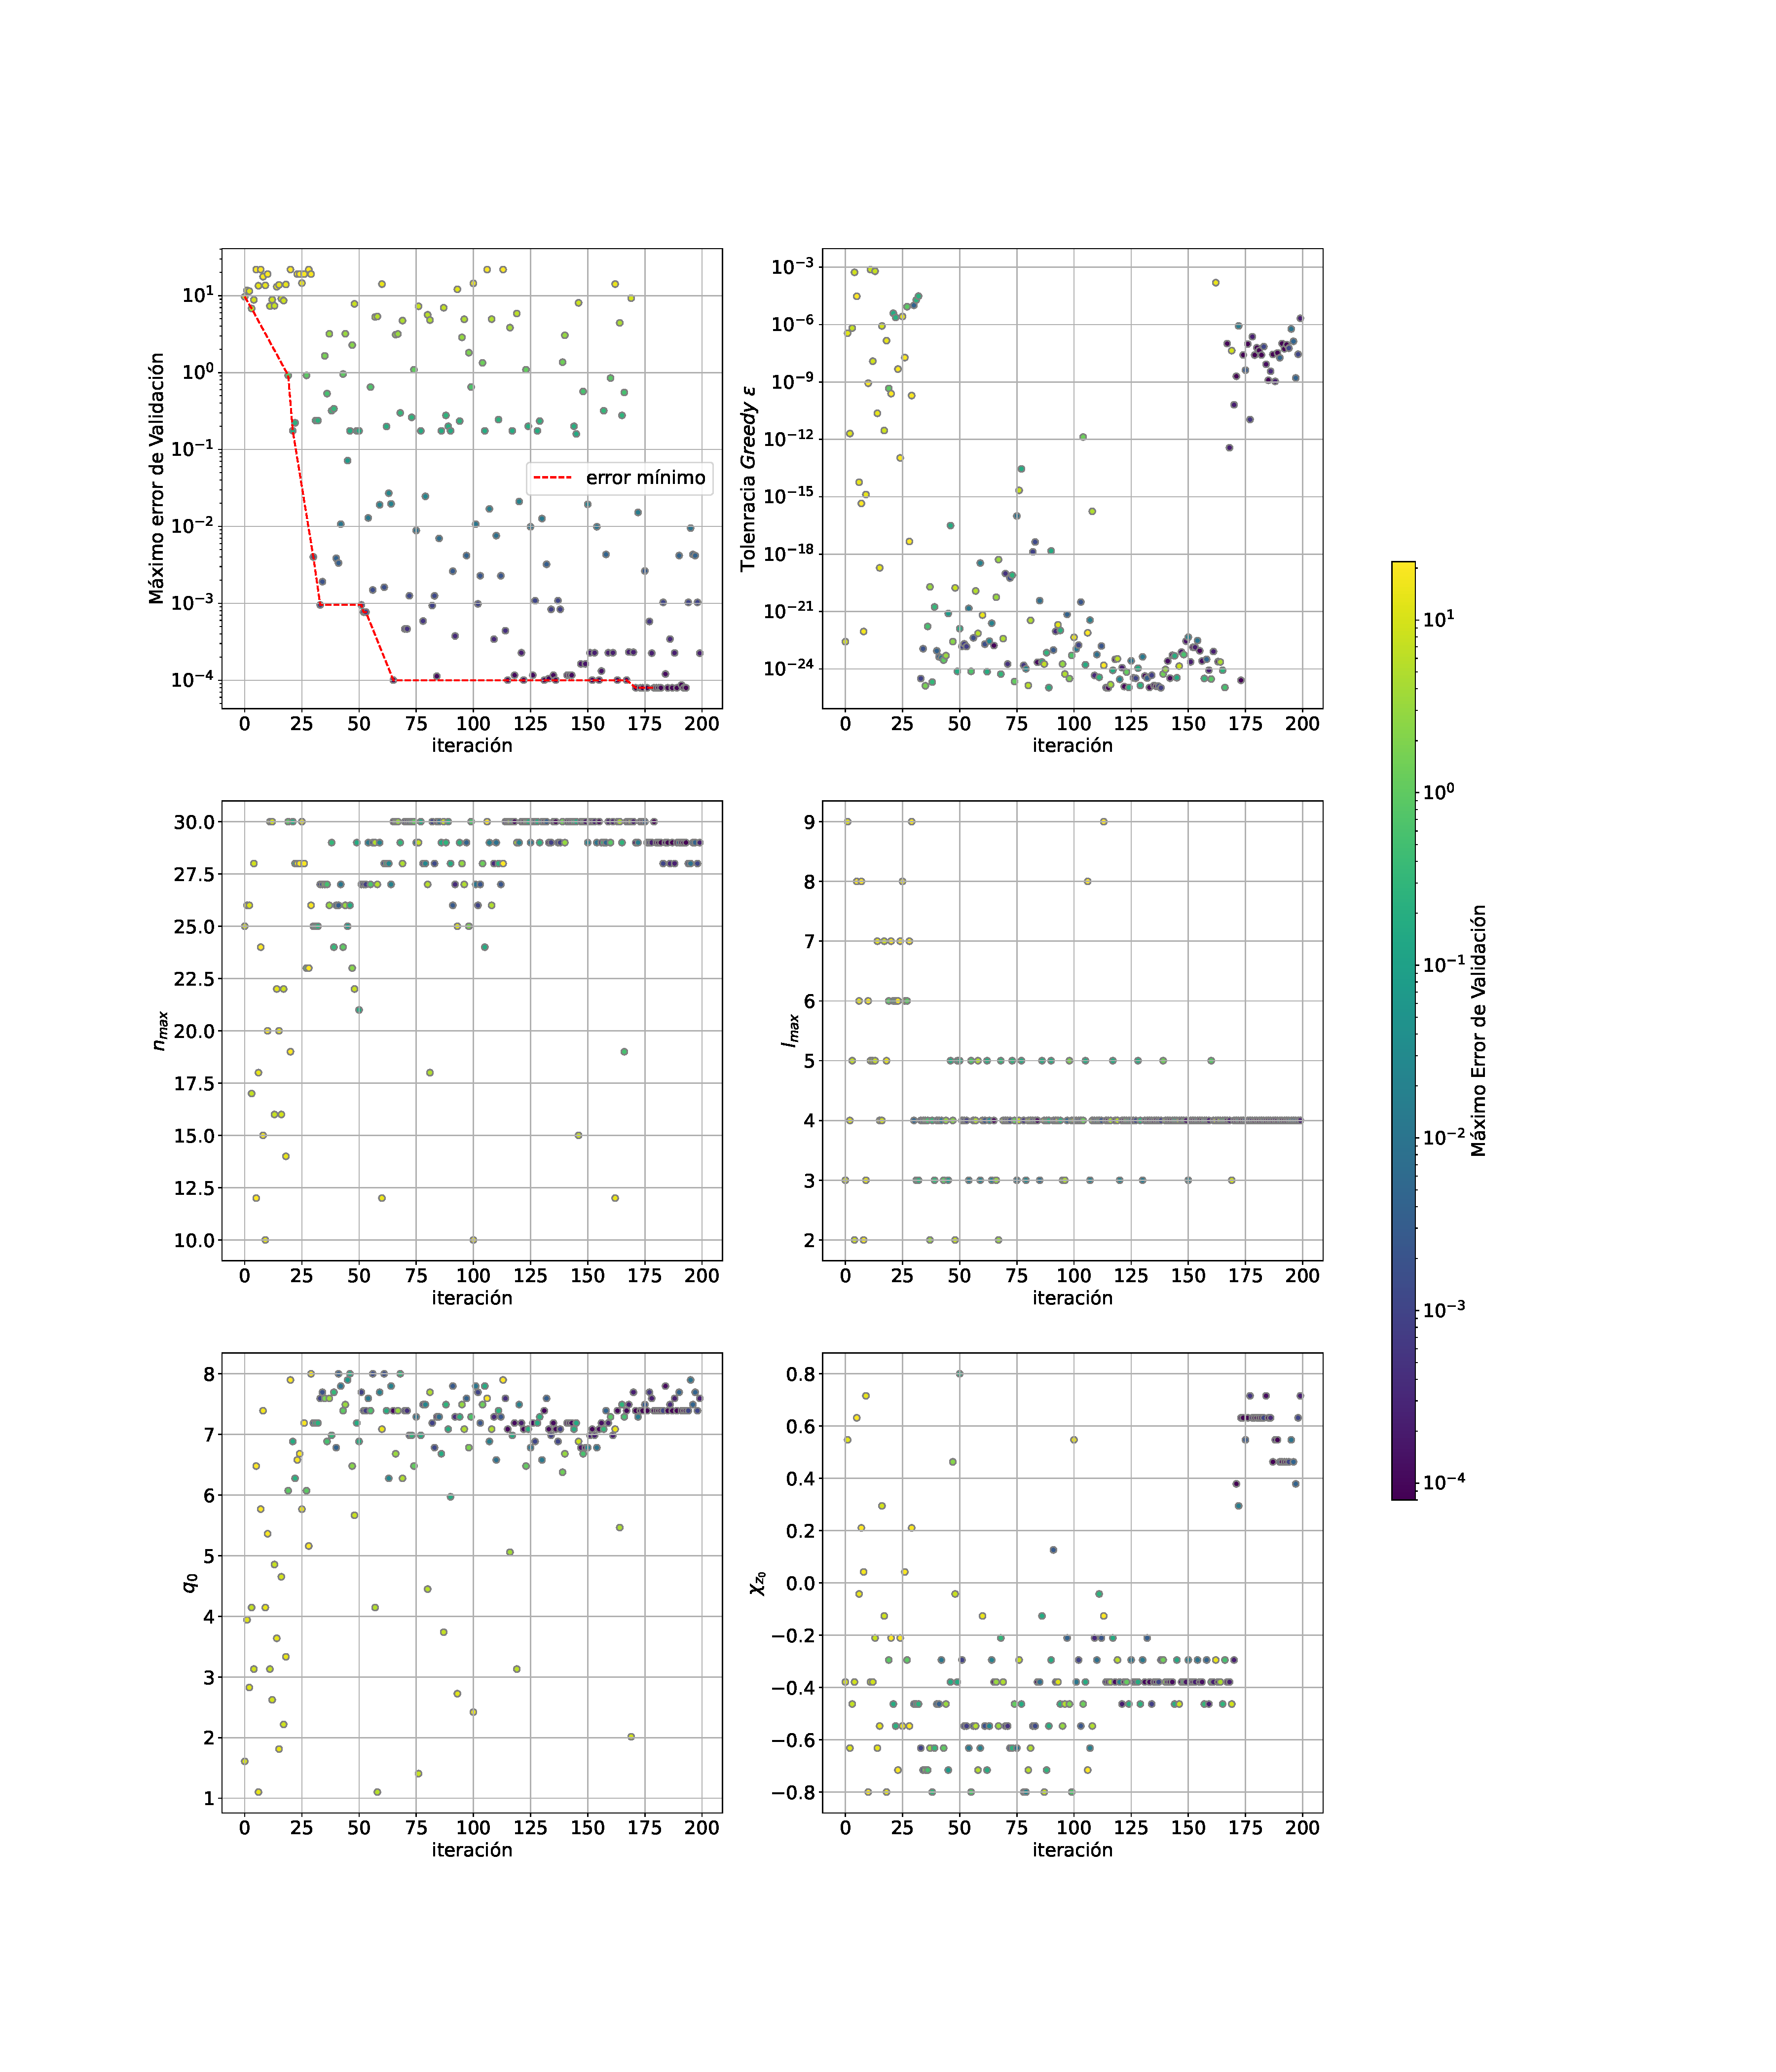
\includegraphics[width=1\columnwidth, trim={6cm, 5cm, 12cm, 5cm}]{Optuna_2D.pdf}
\caption{Optimización con 500 iteraciones para semilla de dos dimensiones utilizando el algoritmo TPE Multivariante.}
\label{fig:optuna_2d}
\end{figure}

Utilizando un conjunto de entrenamiento con 70 valores discretos de $q$ equidistantes en el rango [1, 8] y 20 de $\chi_z$ ($\chi_{z_1} = \chi_{z_2}$) en el rango [-0.8, 0.8], dando lugar a un total de 1400 funciones de onda, se muestran los resultados de optimizar el máximo error de validación utilizando un conjunto de validación con 100 valores para $q$ y 30 vaores para $\chi_z$ con un total de 3000 funciones de onda.

La optimización se realizó en los siguientes espacios de búsqueda:
 
\begin{align*}
n_{max} &\in \{10, 11, 12, ..., 60\},\\
l_{max} &\in \{2, 3, 4, ..., 20 \},\\
\varepsilon &\in \{ 10^{-20}, 10^{-19}, 10^{-18}, ..., 10^{-4}\},\\
Q_0 &= \{ q_0 \ | \ q_0 = 1 + i \Delta q, \ i\in \mathbb{N} : 0 \le i \le 69, \ \Delta q = 7/69 \},\\
X_0 &= \{\chi_{z_0} \ | \ \chi_{z_0} = -0.8 + j \Delta \chi_z, \ j\in \mathbb{N} : 0 \le j \le 19, \ \Delta \chi_z = 1.6/19 \}, \\
\hat{\Lambda}_0 &\in \{ (q_0, \chi_{z_0}) \ | \ q_0 \in Q_0,\ \chi_{z_0} \in X_0 \}.
\end{align*}


En total se realizaron 500 iteraciones, y el mejor máximo error de validación obtenido en la iteración número 269 fue de $1{.}45\times 10^{-6}$ con los hiperparámetros:

\begin{align*}
&n_{max}^* = 59, \\
 &l_{max}^* = 4, \\
&\varepsilon^* = 10^{-17},\\
 &q_0^* = 7.899, \\
 &\chi_{z_0}^* = 0.716.
\end{align*}

En la figura \ref{fig:optuna_2d} se observa la evolución de la optimización realizada, que requirió alrededor de 8 horas para completarse. Se puede ver que para cada hiperparámetro se observa una convergencia a cierto valor, pero sin dejar de lado la exploración, es decir, que se siguen evaluando hiperparámetros fuera del rango que parece óptimo, de forma que se evita caer mucho tiempo en mínimos locales.


\subsubsection{Importancia de los Hiperparámetros}

Una vez realizada una optimización se puede estimar la importancia relativa de cada hiperparámetro con el algoritmo fANOVA \cite{pmlr-v32-hutter14}. Básicamente la idea es dividir la varianza total en distintos componentes que representen la varianza producida por cada hiperparámetro. En la figura \ref{fig:param_import} se observa a la izquierda en naranja los resultados para la optimización realizada, y a la derecha en azul se ven los resultados para otro espacio de búsqueda, esta vez con $n_{max} \in \{20, ..., 30\}$  y $l_{max} = \{2, ..., 8\}$ (es decir que se redujo el espacio de búsqueda para $n_{max}$ y $l_{max}$). Se puede ver que la importancia que tienen los hiperparámetros depende claramente del espacio de búsqueda.

\begin{figure}[h!]
\centering
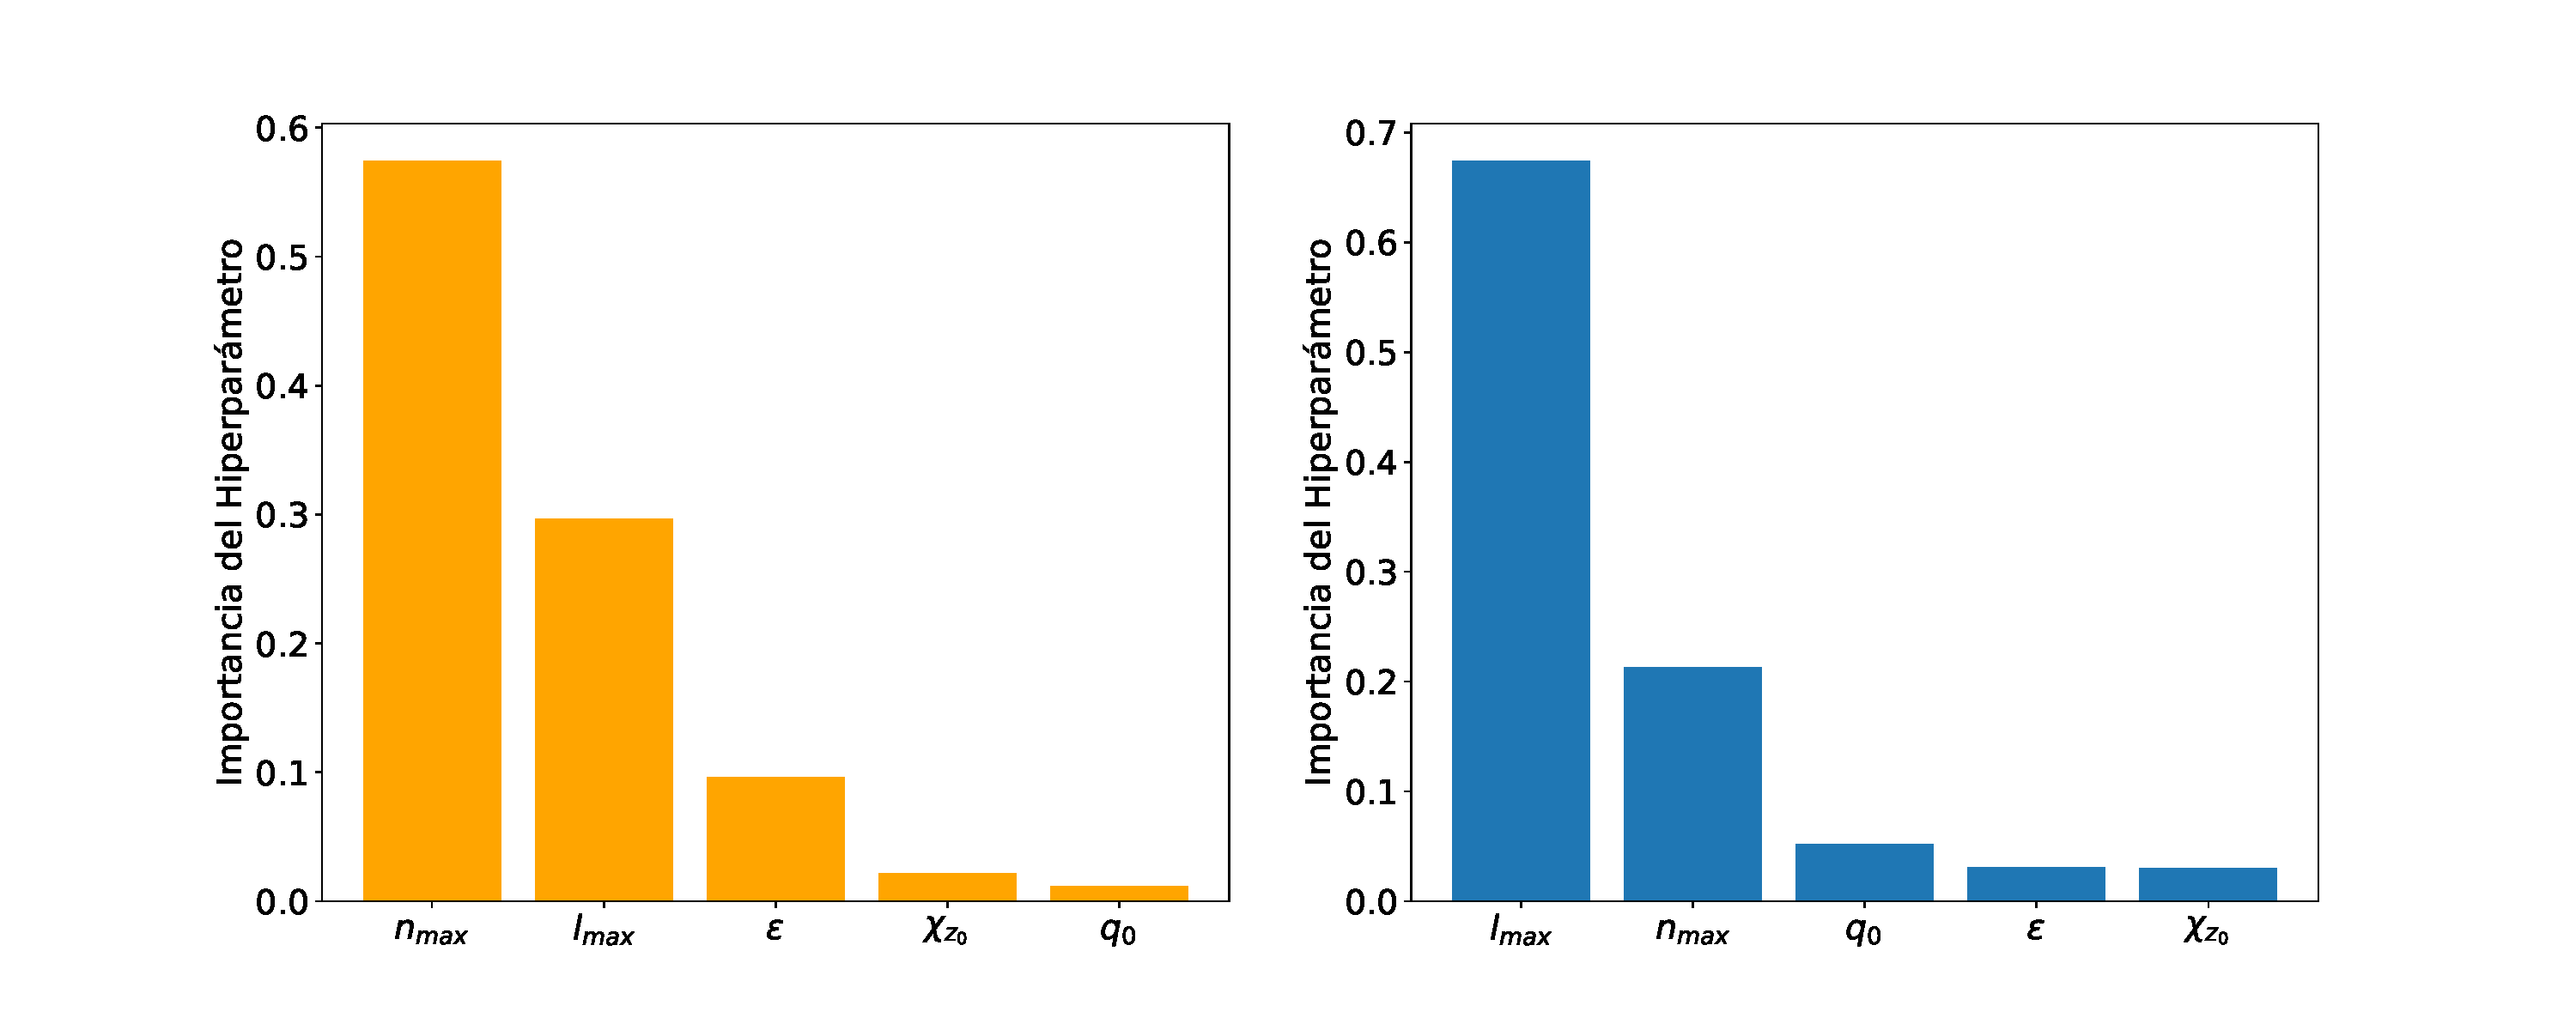
\includegraphics[width=1\columnwidth, trim={5cm, 2cm, 5cm, 2cm}]{params_importance_full.pdf}
\caption{Importancia relativa de los hiperparámetros.}
\label{fig:param_import}
\end{figure}


